\chapter{Capture protocol}

The following document describes the capture protocol proposed for the thesis project Adversarial Anomaly Detector, which aims to be a guide to be followed by potential collaborators. It is important that the collaborator follow this guide in order to have the best data quality for the project.

\section{General considerations}

The data will be captured in the tomato crop field. Typically these plantations are divided into a large number of grooves, so it is intended to create videos that cover each of these grooves. The distance between the groove ranges from 1.8 to 2 meters. Figure [FIGURE] shows an example of a tomato plantation.

\begin{figure}[htb]
  \centering
  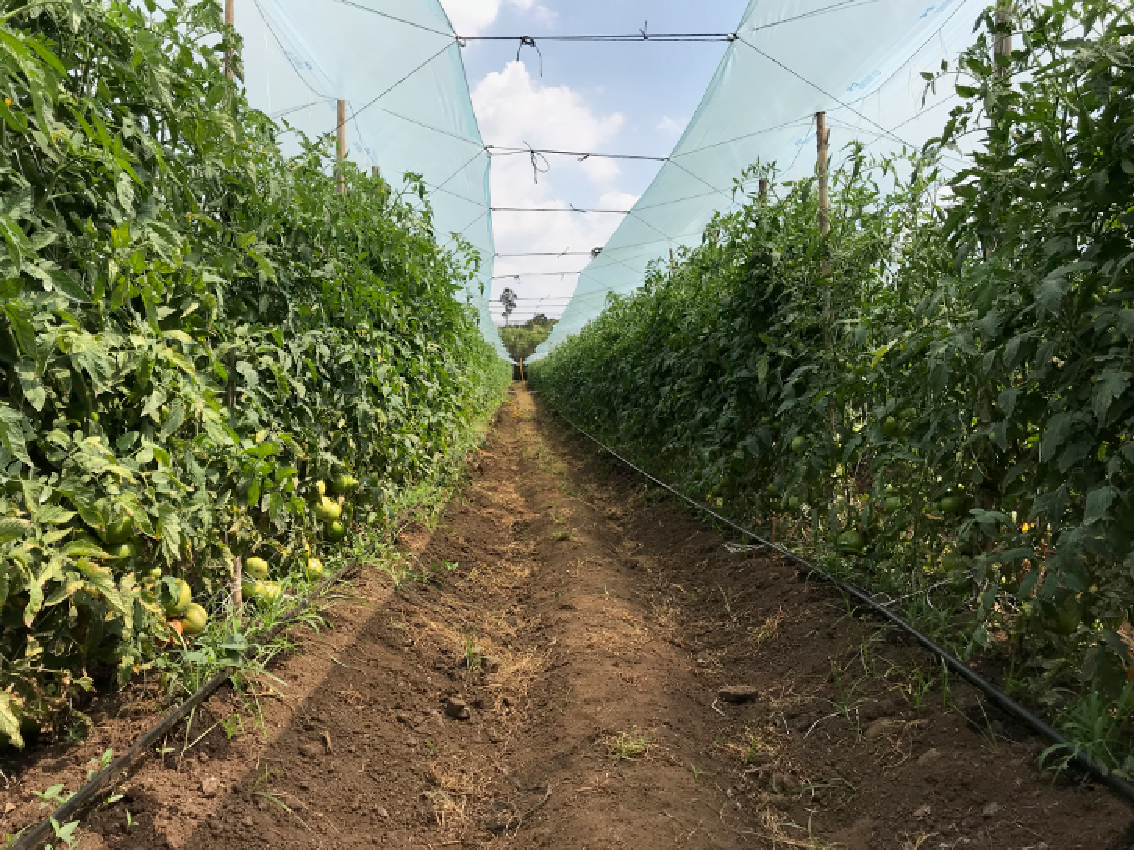
\includegraphics[width=100mm]{tomato_crop}
  \caption[Tomato crop]{Tomato crop in Costa Rica.}
  \label{fig:tomato_crop}
\end{figure}

\section{Video considerations}

\begin{itemize}
 \item The video resolution must be 1920x1080 pixels.
 \item Make use of a video stabilizer like a Gimbal. (For example the DJI Osmo Mobile 2)
 \item The video must be recorded in color.
 \item The duration of the video will depend on the length of the groove.
 \item The distance of the chamber from the plants should be approximately 1.5 meters.
 \item The video should cover the entire structure of the plant, from its base to the highest branches. If it is not possible to cover the entire plant in the same video, it will be done in different videos, covering in one of them the upper part of the plant and in another the lower part.
 \item Use the camera of a cell phone with Android or iOS operating systems.
 \item Use a mobile application that is capable of controlling the cell phone's front camera. Suggested applications: Filmic Pro.
 \item Utilizar una tarjeta de calibración de color previo a realizar los videos.
\end{itemize}

\section{Instructions for capturing the video}

As mentioned earlier, the videos cover each groove that confirms tomato plantations. Below are instructions to correctly capture the videos:

\begin{figure}[htb]
  \centering
  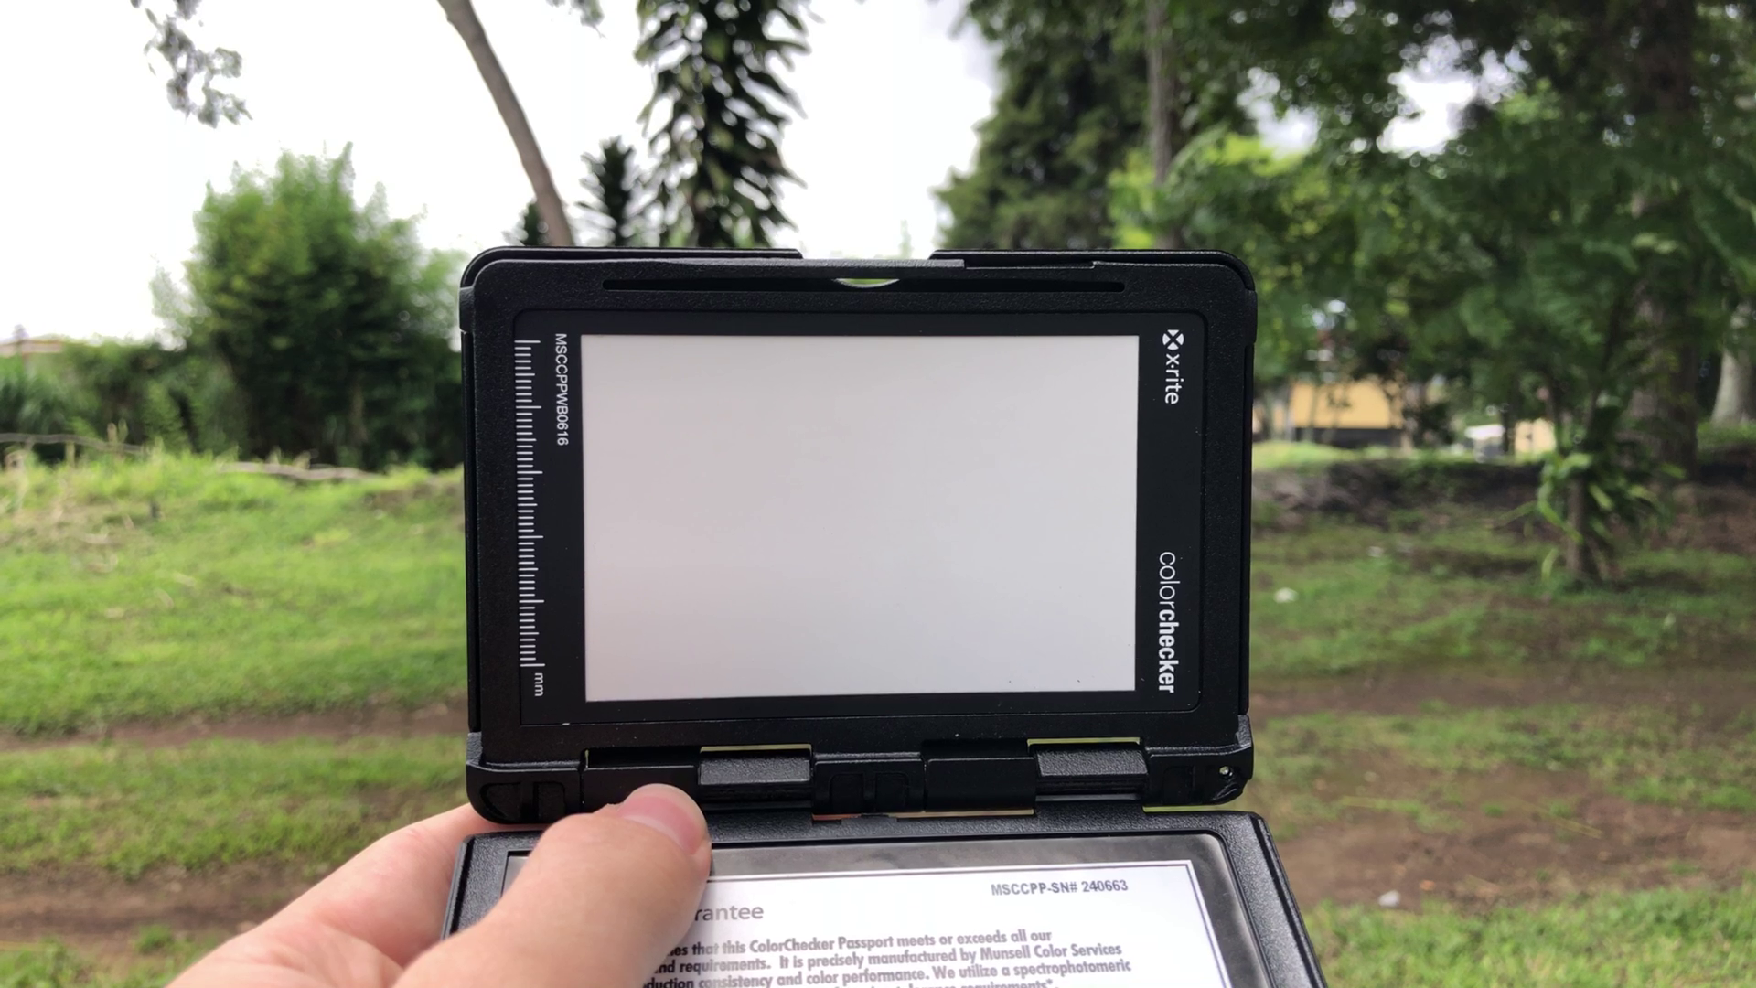
\includegraphics[width=100mm]{protocol2}
  \caption[Color calibration]{Colo checker gray card.}
  \label{fig:color_calibration}
\end{figure}

\subsection{Color calibration}

Using a gray scale calibration card, the camera's white balance should be adjusted as follows.

\begin{enumerate}
 \item Enter to the Filmic Pro application.
 \item Position the calibration card in front of the camera and zoom in to focus on the card only.
 \item Go to the camera settings and select the section related to white balance.
 \item Select the option to perform an automatic white balance.
 \item Wait a moment for the camera's white balance to be automatically adjusted and then select the option to set the white balance.
 \item It is important to mention that this process must be carried out in the place where the capture is intended and it is also recommended to repeat the steps every 30 minutes, to anticipate possible changes in the lighting that the place presents.
\end{enumerate}

\begin{figure}[H]
\begin{minipage}{\linewidth}
  \centering
  \begin{tabular}{ccc}
  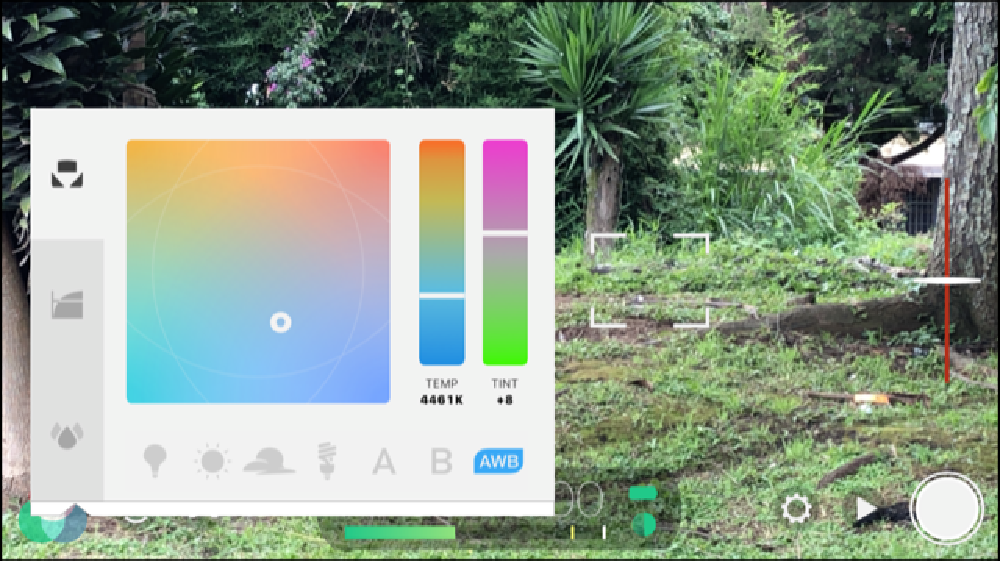
\includegraphics[width=.40\linewidth]{protocol4}
    & 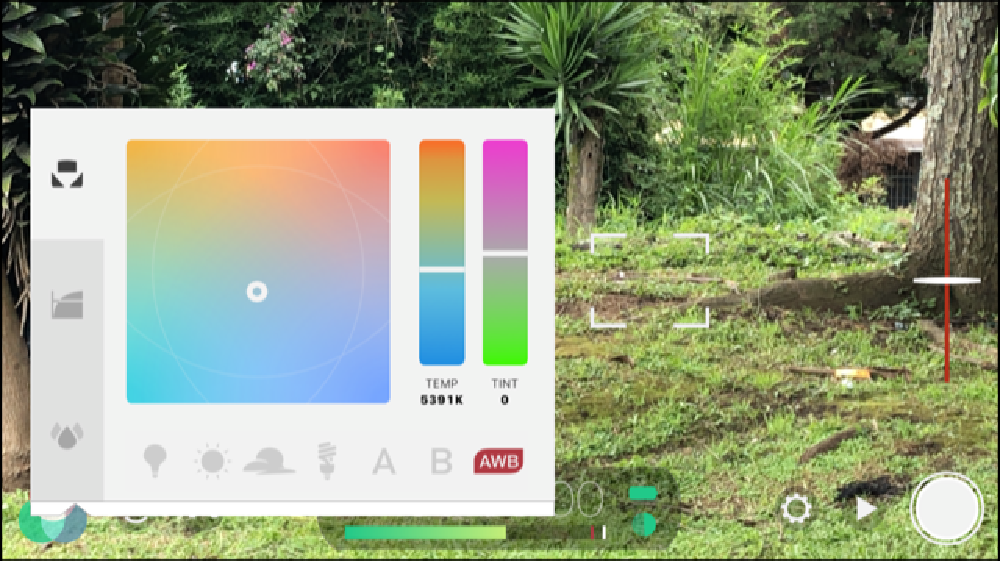
\includegraphics[width=.40\linewidth]{protocol5} \\
  (a) & (b) 
  \end{tabular}
  \end{minipage}
\caption[Whitebalance configuration]{Whitebalance configuration: In a) the automatic white balance is displayed and in b) the fixed white balance.}
\label{fig:whitebalance}
\end{figure}

\subsection{Proper use of the gimbal}

The following are some recommendations for optimal use of the gimbal.

\begin{enumerate}
 \item Make use of a tripod that allows you to make a gimbal grip with both hands.
 \item Tilt the device slightly forward in order to have greater stability during video capture.
 \item Make slow and constant movements. The suggested way of walking with the gimbal is to slightly bend the knees to have greater cushioning of the steps and avoid sudden movements of the camera.
\end{enumerate}

\subsection{Pre-capture application settings}

In order to avoid as much as possible the effect of blurring that can cause the taking of a moving video, it is recommended to set the frame rate of the application to 120 FPS and thus achieve a slow motion effect.

